 
\documentclass[a4paper, 12pt]{article}
 
\usepackage[margin=1in]{geometry} 
\usepackage{amsmath,amsthm,amssymb}
\usepackage{titlesec}
\usepackage{graphicx}
\usepackage{float}

\titleformat{\section} {\normalfont\large\bfseries}{\thesection}{1em}{}
\titleformat{\subsection} {\normalfont\large\itshape}{\thesection}{1em}{} 

\begin{document}
 
\title{Otto Group Product Classification Challenge}
\author{Machine Learning Project\\Prof. Ulrike von Luxburg\\ TA. Morteza Alamgir} 
\date{June 17, 2015}
 
\maketitle

\section*{Challenge Overview} 

	This challenge was sponsored by the Otto group, one of the biggest e-commerce companies with headquarters in Hamburg, Germany. Their operations involve the managing of thousands of products to be sold worldwide on a daily basis. Therefore, correctly identifying and classifying these products is of utmost importance. \\
The objective of this challenge is to create a predictive model which is able to distinguish between their main product categories (9 in total).
Two data sets were provided: a train set, with information for 61 878 products, and the test set, consisting of 144 368 products. Both data sets are structured like in table \ref{Tab: Struc}. There are a total of 93 numerical features, which represent counts of different events. No further details were given about to what each feature corresponds.

 \begin{table}[H]
 \centering
 \caption{Data Set Structure} \label{Tab: Struc}
 \begin{tabular}{|c |c c c| c|} 
  \hline
 Product Id & Feat 1  & \ldots & Feat 93 & Target \\ [0.5ex] 
 \hline
 1 & 0 & \ldots & 24 & Class 1\\
 \vdots & \vdots & \vdots & \vdots & \vdots\\ 
  61 878 & 1 & \ldots & 1 & Class 9\\
 [1ex] 
 \hline
\end{tabular}
 
\end{table} 

\section*{Data Analysis}

As previously mentioned, the train set consists of 93 feature information for each of the 61 878 products, classified into 9 different classes. The train data set is formed with unbalanced classes as shown on fig. \ref{fig:Dist}
%I uploaded my matlab file, in case you

		\begin{figure}[H]
            \centering 
            \includegraphics[width=\textwidth]{Class-DataPointDist}
            \caption{Data Points per Class}
            \label{fig:Dist}
		\end{figure}

\subsection*{Statistics} %Maybe its best not to place subsections 

Figure \ref{fig:FDstacked} shows t

		\begin{figure}[H]
            \centering 
            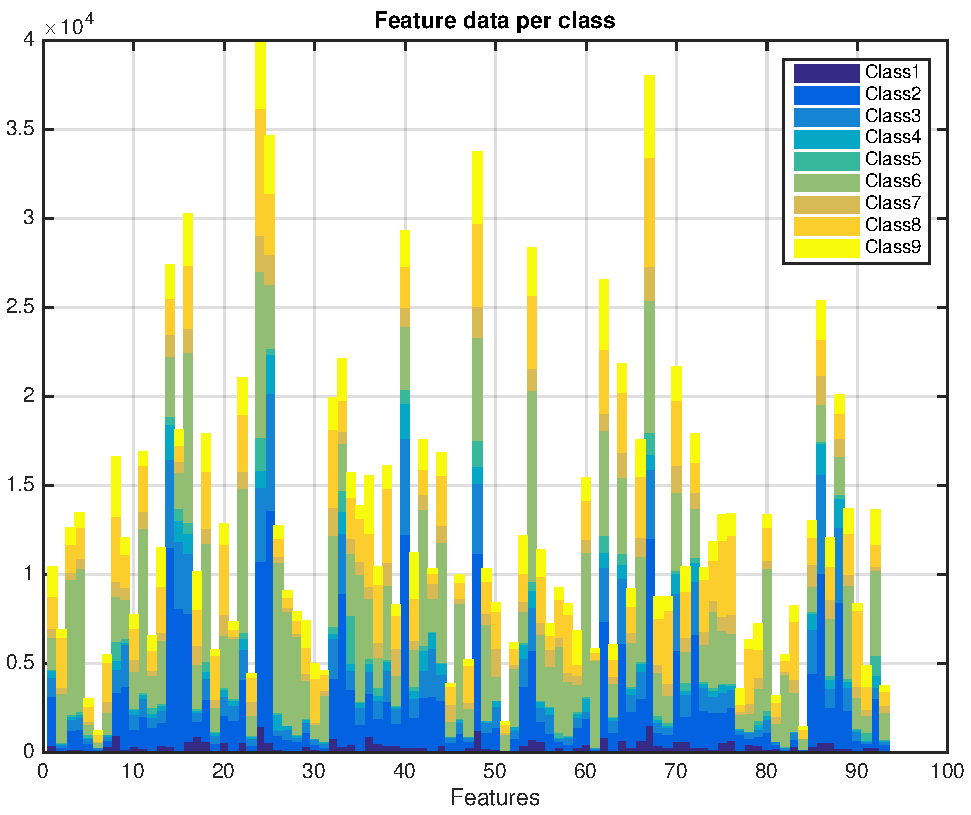
\includegraphics[width=\textwidth]{Feature_Data_stacked}
            \caption{Feature Distribution per Class}
            \label{fig:FDstacked}
		\end{figure}


\subsection*{Dimensionality-Reduction}
\subsection*{Clustering}


\pagebreak
\section*{Appendix}
\subsection*{Appendix A - Class vs Feature Plots}

		\begin{figure}[H]
            \centering 
            \includegraphics[width=\textwidth]{ClassvsFeature1_32}
            \caption{Class vs Features (1-32)}
            \label{fig:CF1_32}
		\end{figure}

		\begin{figure}[H]
            \centering 
            \includegraphics[width=\textwidth]{ClassvsFeature33_64}
            \caption{Class vs Features (33-64)}
            \label{fig:CF33_64}
		\end{figure}
        
		\begin{figure}[H]
            \centering 
            \includegraphics[width=\textwidth]{ClassvsFeature65_93}
            \caption{Class vs Features (65-93)}
            \label{fig:CF65_93}
		\end{figure}

\subsection*{Appendix B - Feature vs Class Plots}

		\begin{figure}[H]
            \centering 
            \includegraphics[width=\textwidth]{FeaturevsClass1_3}
            \caption{Feature vs Class (1-3)}
            \label{fig:FC1_3}
		\end{figure}

		\begin{figure}[H]
            \centering 
            \includegraphics[width=\textwidth]{FeaturevsClass4_6}
            \caption{Feature vs Class (4-6)}
            \label{fig:FC4_6}
		\end{figure}
        
		\begin{figure}[H]
            \centering 
            \includegraphics[width=\textwidth]{FeaturevsClass7_9}
            \caption{Feature vs Class (7-9)}
            \label{fig:FC7_9}
		\end{figure}









\end{document}